%% Juan Luis Padilla Salome <jps55@alumnos.unican.es>

\documentclass[a4paper, 12pt]{report}


\usepackage[utf8]{inputenc}
\usepackage{graphicx}
\graphicspath{ {images/} }

% Packages to use
% % Packages you intend to use
% ..

% For example, if you want to render 
% the document in a different font you can
% use something like: 

% \usepackage{gentium}

\usepackage{url}

% start
% --------------------------
\begin{document}

% Portada

\begin{titlepage}
    \begin{center}
        \vspace*{1cm}
 
        
\includegraphics[height=3.8cm]{logo_UC.png}

        \vspace{1.0cm}

        \Large
        \textbf{Facultad de Ciencias}

        \vspace{1.0cm}

        \LARGE
        \textbf{An\'alisis de rendimiento de aplicaciones de Deep Learning (Keras) sobre procesadores de prop\'osito general}
 
        \vspace{0.3cm}

        \Large
        Performance analysis of Deep Learning applications (Keras) on general purpose processors

        \vspace{1.5cm}

        \large
        Trabajo de Fin de Grado para acceder al

        \vspace{0.8cm}

        \Large
        \textbf{GRADO EN INGENIERÍA INFORMÁTICA}
 
        \vfill

        \large
        \begin{flushright}
            \textbf{Autor: Juan Luis Padilla Salomé}

            \vspace{0.4cm}

            \textbf{Director: Pablo Abad Fidalgo}

            \vspace{0.6cm}

            Junio 2021
        \end{flushright}
             
    \end{center}
 \end{titlepage}











% Make the title. You can pass an option to this
% to render the title differently, like so:
%\maketitle[logo-first]
% \maketitle

% And so begins the thesis! First include pages
% before the acknowledgements
% The blank page environment allows you to insert
% pages into your thesis for specific things

\clearpage\null\newpage


% Acknowledgements

\renewcommand{\abstractname}{Acknowledgements}
\begin{abstract}
    Thanks!
\end{abstract}

% The abstract of the thesis
\begin{abstract}
Here is the abstract for this thesis.
\end{abstract}

% Print out the table of tables and table of figures and
% tell the template we're about to start the body of the
% thesis.
% \thesisTables
% \thesisBodyStart


% start of thesis body
% ---------------------------

% Include introduction
% \chapter{Introduction}
% Intro + motiv
Hello world

% Related work 
% \chapter{Related Work}
...
\cleardoublepage
...

% Method
% \chapter{Method}
Here is a sentence, and you can see a nice picture in Figure \ref{fig:brayford}.

\begin{figure}[h]
    \centering
    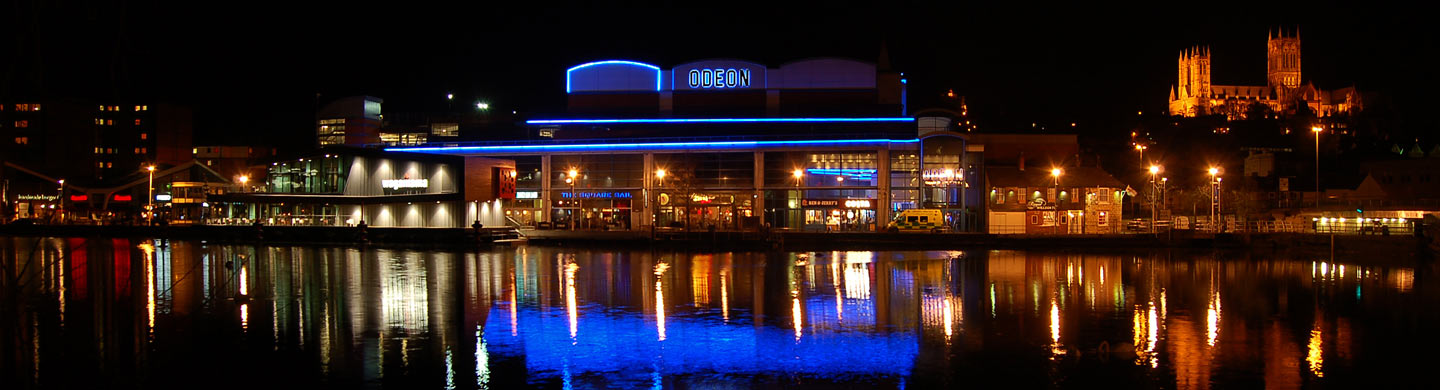
\includegraphics[width=\textwidth]{figures/brayford.jpg}
    \caption{A picture of the Brayford from Google Images.}
    \label{fig:brayford}
\end{figure}

Also, a table can be found in Table \ref{tbl:example-table}. You should use a \LaTeX~table generator like \url{https://www.tablesgenerator.com/} if you want to make your life easier.

\begin{table}[h]
    \caption{Here is a table. The caption goes above like this.}
    \centering
    \begin{tabular}{l|l|c}
        First name & Last name & Age \\
        \hline\hline
        Bob & Bobbington & 24 \\
        Benth & Wavies & 49 \\
        Joe & Bloggs & 37 \\
        Billy & Bob & 10 \\

    \end{tabular}
    \label{tbl:example-table}
\end{table}

% Conclusions
% \chapter{Conclusions}
...


% end of thesis body
% --------------------------

% Print out the references
% \printReferences

% Print out the ludography (optional)
% \printLudography

% If you want to put some text before the list of games,
% then you can use the following code:
%\begin{ludography}[Ludography / Optional Title]
    %Here are some games.
%\end{ludography}


\end{document}
